% additional use of \usepackage{beamerthemesplit}
\documentclass{beamer}
\usepackage{beamerthemesplit} % new 
\usepackage{hyperref}
\usepackage{multimedia}
\usepackage{animate}
\usepackage[export]{adjustbox}


\definecolor{verde}{rgb}{0.5,1,0.2}
\definecolor{rojo}{rgb}{1,0,0}
\definecolor{azul}{rgb}{0,0,1}

\begin{document}

\title{Machine Learning techniques applied to cosmological problems.} 
\author{Mart\'in de los Rios} 
\date{}

\frame{
  \titlepage
  Director: Dr. Mariano Dom\'inguez
} 

\frame{
  \tiny
  \frametitle{Resumen}
  \tableofcontents
} 

\section{Introduction to Machine Learning techniques.}

\frame{
\tableofcontents[ 
    currentsubsection, 
    sectionstyle=show/hide, 
    sectionstyle=show/shaded, 
    ] 
}

\frame{
  \frametitle{Supervised Learning.}
  \begin{center}
   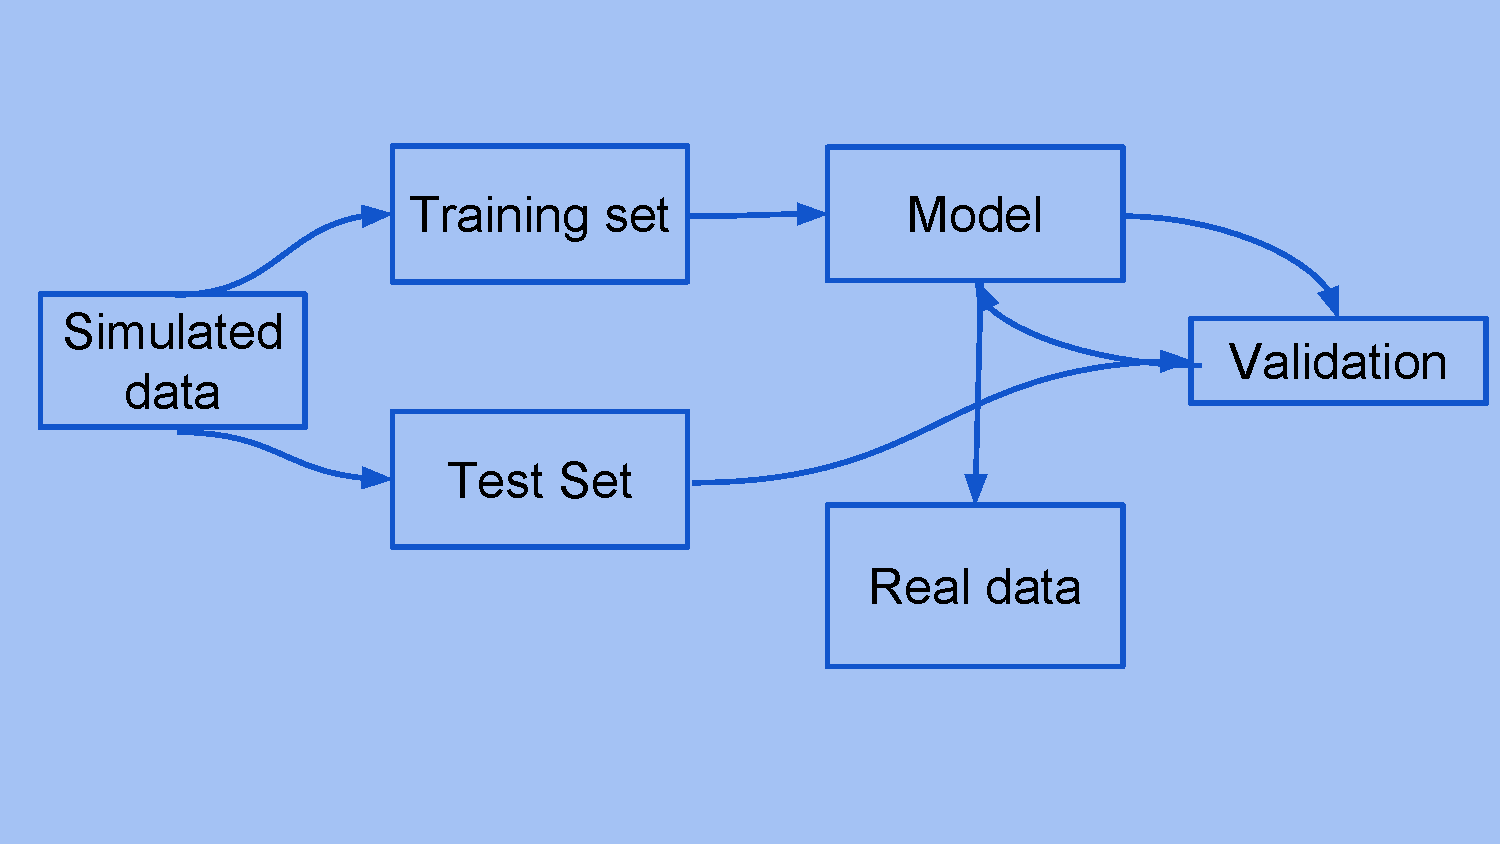
\includegraphics[scale=0.45]{./aprendizaje_supervisado.pdf}
  \end{center}
}

\begin{frame}{Random Forest}
  \animategraphics[loop,controls,scale=0.3]{10}{random_forest-}{0}{20}
\end{frame}

\frame{
  \frametitle{Random Forest}
  \begin{center}
 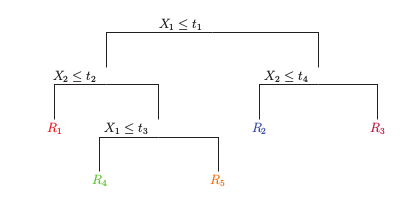
\includegraphics[scale=0.85]{./rf.png}
 % rf.png: 0x0 pixel, 300dpi, 0.00x0.00 cm, bb=
\end{center}

}

\begin{frame}{Support Vector Machines}
  \animategraphics[loop,controls,scale=0.3]{10}{support_vector_machines-}{0}{40}
\end{frame}

\frame{
  \frametitle{Support Vector Machine}
  \begin{center}
 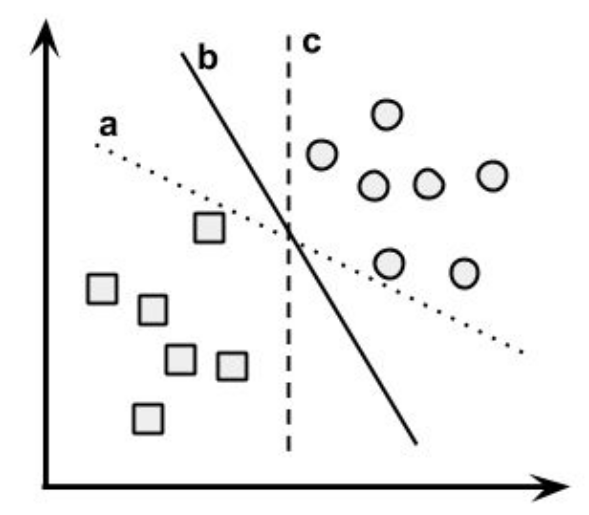
\includegraphics[scale=0.4]{./svm.png}

 % svm.png: 0x0 pixel, 300dpi, 0.00x0.00 cm, bb=
\end{center}

}

\frame{
  \frametitle{Unsupervised Learning.}
  \begin{center}
 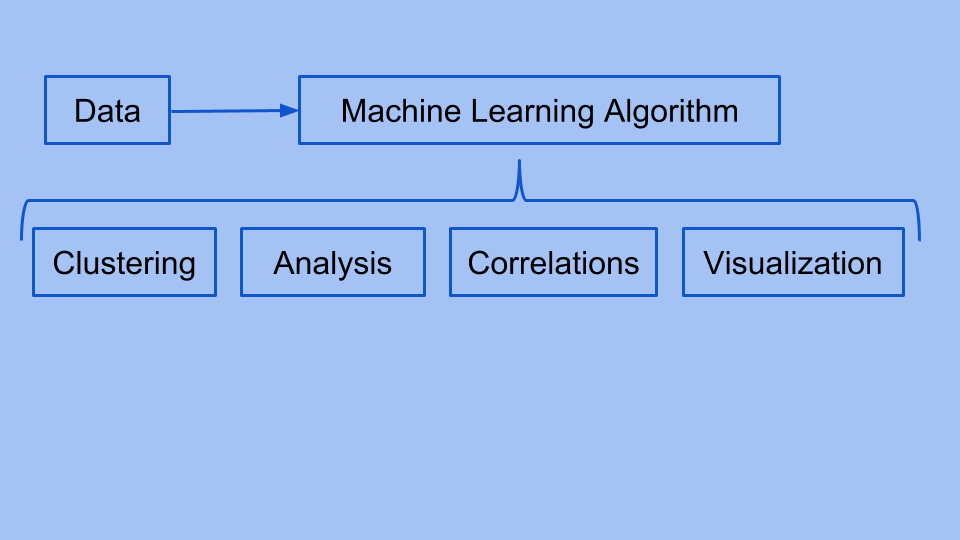
\includegraphics[scale=0.34]{./aprendizaje_nosupervisado.png}
 % aprendizaje_nosupervisado.jpg: 0x0 pixel, 300dpi, 0.00x0.00 cm, bb=
\end{center}

}

\begin{frame}{Mixture of Gaussians}
  \animategraphics[loop,controls,scale=0.3]{10}{mixture_of_gaussians-}{0}{14}
\end{frame}

\frame{
 \frametitle{Mixture of Gaussians.}
 \begin{center}
 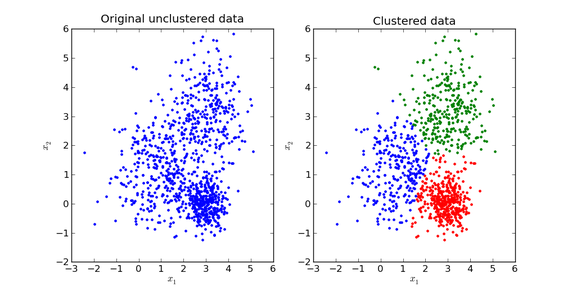
\includegraphics[scale=0.5]{./mixt_gauss.png}
 % mixt_gauss.png: 0x0 pixel, 300dpi, 0.00x0.00 cm, bb=
\end{center}
}
\frame{
\frametitle{Principal Components Analysis.}
\begin{center}
 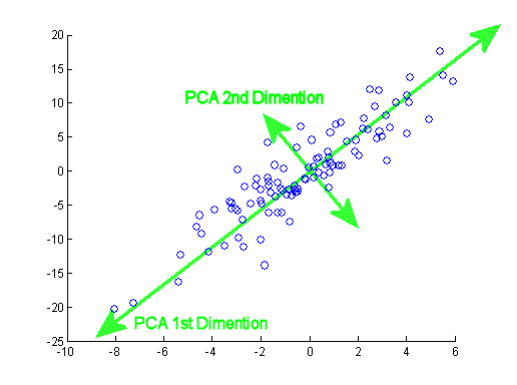
\includegraphics[scale=0.5]{./pca.png}
 % pca_example.gif: 0x0 pixel, 300dpi, 0.00x0.00 cm, bb=
\end{center}

}

\section{The \texttt{MeSsI} (Merging Systems Identification) Algorithm.}

\frame{
\tableofcontents[ 
    currentsubsection, 
    sectionstyle=show/hide, 
    sectionstyle=show/shaded, 
    ] 
}

\section{Analysis of individual merging clusters candidates.}

\frame{
\tableofcontents[ 
    currentsubsection, 
    sectionstyle=show/hide, 
    sectionstyle=show/shaded, 
    ] 
}

\subsection{A2029/2033.}
\subsection{A1204.}
\subsection{A267.}
\subsection{Statistical analysis of the magnetic fields in merging clusters.}

\section{\texttt{CosmoMl}:Machine Learning techniques applied to the CMB.}

\frame{
\tableofcontents[ 
    currentsubsection, 
    sectionstyle=show/hide, 
    sectionstyle=show/shaded, 
    ] 
}

\subsection{Construction of the data set.}
\subsection{Unsupervised methods.}
\subsection{Supervised methods.}
\subsection{Cosmological parameters Angular distributions.}

\section{Conclusions.}

\frame{
\tableofcontents[ 
    currentsubsection, 
    sectionstyle=show/hide, 
    sectionstyle=show/shaded, 
    ] 
}


\frame{
\begin{figure}[ht!]
 \centering
 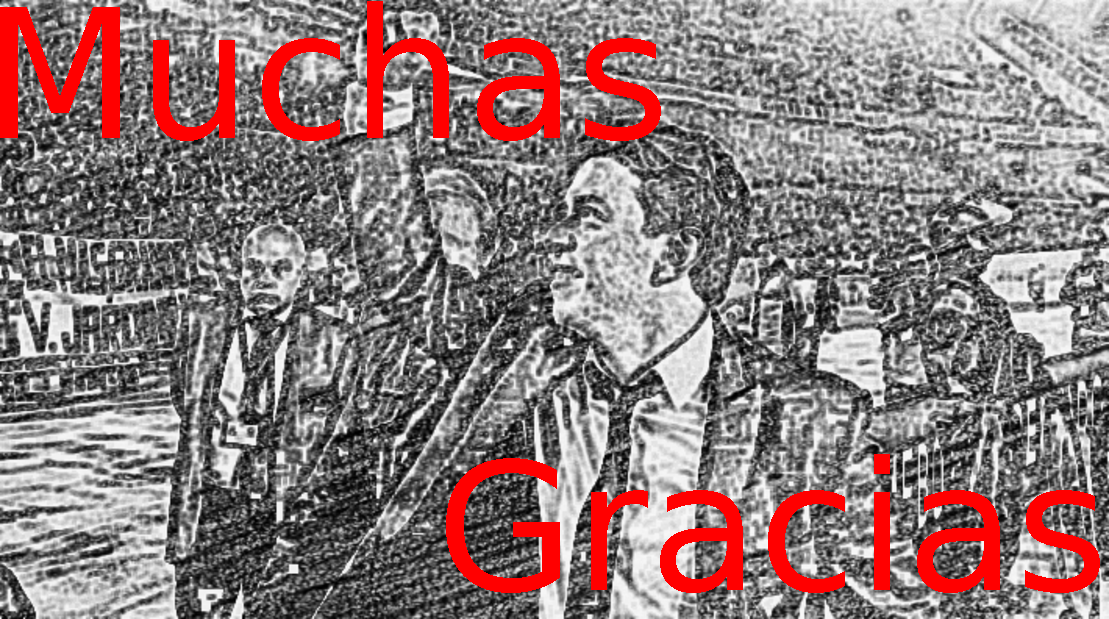
\includegraphics[scale=0.63]{./gracias2.pdf}
% nfw_velocity_distributions.pdf: 0x0 pixel, 300dpi, 0.00x0.00 cm, bb=
\end{figure}
}
\end{document}

